\section{A Primer on Lagrangian Mechanics}

\subsection{Motivation}
In one's typical formal education, the study of mechanics often begins with Newton's laws, which describe the motion of objects via forces $\sum_i F_i$ and accelerations. However, Lagrangian mechanics provides a powerful alternative framework, especially well-suited for systems with constraints and generalized coordinates. In Newtonian mechanics, introducing a constraint involves determining the precise forces which need to act on an object to ensure the constraint is satisfied. In Lagrangian Mechanics, one does not require to engineer such subtleties, and can rather define any coordinates they wish to describe the system, some which for example may implicitly take the constraint into account.

\begin{figure}[H]
	\centering
	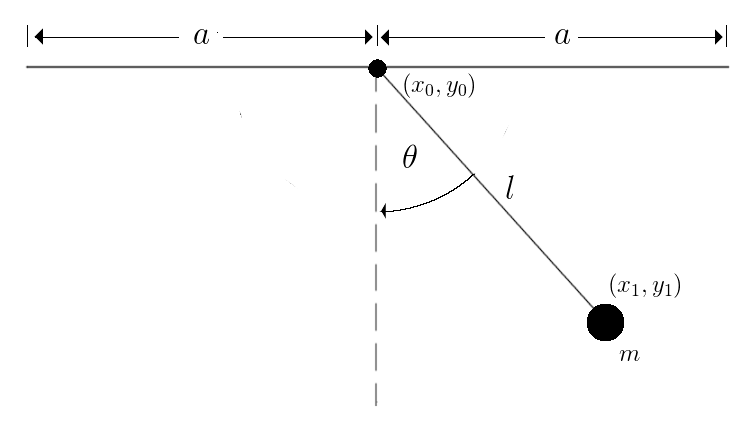
\includegraphics[width=0.5\textwidth]{assets/simple_pendulum.png}
	\caption{A simple pendulum, illustrating the use of generalized coordinates $(x_1,y_1)\to\theta$ (RlGuy).}
	\label{fig:simple_pendulum}
	% Source: https://rlguy.com/lagrangeexample/
\end{figure}

Consider the example of the simple 2D pendulum of length $l$. In Newtonian mechanics, one may have defined this system in terms of the bobs $x$ and $y$ coordinates. Since the length of the rod is fixed, it would be necessary to find a way to solve for the dynamics while also imposing the constraint that $\sqrt{x^2+y^2}=l$. Then, while simultaneously taking this constraint into account, one would need to determine the total force on the bob as a sum of the tension $\vec T$ and the gravity $\vec g$. In the end, this becomes quite complicated, and warrants the use of some nontrivial forces expressed in $x$ and $y$. With \textbf{Lagrangian Mechanics} on the other hand, we can pick our coordinates more freely, indirectly taking the constraints into account. For example, we could take the angle made of the bob from the vertical, $\theta$, as our coordinate. Then, using the Lagrangian toolkit, we simply figure out what the kinetic and potential energy of the system is with respect to this coordinate, and all equations of motion immediately follow.

\subsection{The Principle of Stationary Action and Calculus of Variations}

The central object in Lagrangian mechanics is the \textbf{Lagrangian function}.

\begin{smjdefinition}[The Lagrangian Function]{lagrangianfunction}
	The Lagrangian $L:\mathbb{R}^{2n+1}\to\mathbb{R}$ is defined as the difference in potential and kinetic energy, $T$ and $V$,
	$$L(q_1, q_2, \ldots, q_n, \dot{q}_1, \dot{q}_2, \ldots, \dot{q}_n, t) = T(\dot q_1, \ldots, \dot q_n) - V(q_1, \ldots, q_n).$$
\end{smjdefinition}

\vspace{1em}

The Lagrangian function is extremely important in considering physical systems, as it is a crucial component of one of the most important quantities in physics: the \textbf{action functional} $\mathcal{S}(L)$. 

\begin{smjdefinition}[The Action Functional]{actionfunctional}
	The action functional $\mathcal{S}(L)$ maps the Lagrangian function to some scalar quantity, representative of some average difference in potential $V$ and kinetic energy $T$ over a time interval $[t_1,t_2]$.
	$$\mathcal{S}(L)=\int_{t_1}^{t_2} L(q_1,\ldots,q_n, \dot q_1, \ldots, \dot q_n, t)dt$$
\end{smjdefinition}

In physics, one may think of the action $\mathcal{S}(L)$ as a measure of the balance of kinetic and potential energy throughout a systems trajectory. Mathematically however, it can be thought of as a \textbf{functional} with the Lagrangian function $L$ as its argument. 

\begin{smjdefinition}[Functional]{functional}
	A functional is an object which lives in the \textbf{dual space} of the normed vector space of functions. In other words, it is a map that takes in a given function, and returns a scalar. Unlike a usual function, which maps scalar to scalar, or vector to scalar, a functional maps an entire function to a scalar. Examples of functionals include: definite integrals, taking the maximum/minimum, the $\mathcal{L}^p$ norm, etc.
\end{smjdefinition}

As the name suggests, the action functional is a functional. Particularly, it takes in the Lagrangian function of a given physical system evolving over a time interval $[t_1,t_2]$, and returns a single value representative of the energy fluctuation between kinetic and potential over time. While such a quantity may not immediately pose itself as extremely useful, it singlehandedly underpins much of our understanding of the physical universe, as it obeys one of the most important principles in semi-modern physics: the \textbf{principle of stationary action}. 

\begin{smjdefinition}[The Principle of Stationary Action]{stationaryaction}
	This principle states that the trajectory of a real world physical system $(q_1(t),\ldots, q_n(t))$ always yields a Lagrangian function $L$ which results in a \textbf{stationary output} of the action functional $\mathcal{S}$. Namely, the \textbf{variation $\delta$} of the action functional is zero:
	$$\delta S = 0$$
\end{smjdefinition}

To fully understand what this principle implies, let us define the concept of the variation of a function, which in as sense can be thought of as the infinitiesimal change of a functional with respect to its function argument.

\begin{smjdefinition}[The Variation of a Functional]{variationfunctional}
	The variation of a functional is defined as an infinitesimal perturbation of a function. Let $\eta(x)$ be an arbitrary function that admits at least one derivative, and let $\varepsilon\in\mathbb{R}, |\varepsilon| \ll 1$. Then, the variation of a functional $\mathcal{S}(L)$ is given by:
	$$\delta \mathcal{S}=\mathcal{S}(L+\varepsilon\eta)$$
\end{smjdefinition}

\begin{figure}[H]
	\centering
	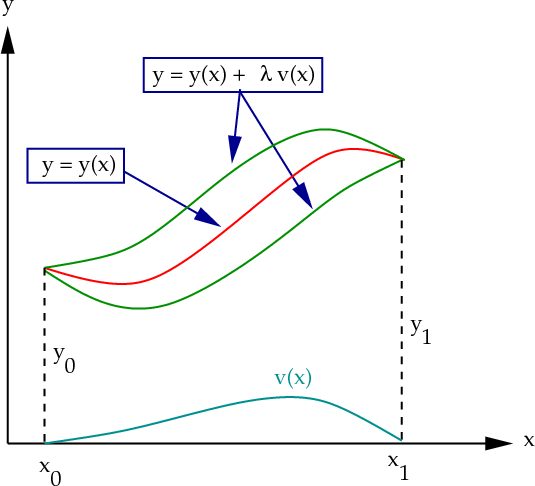
\includegraphics[width=0.5\textwidth]{assets/functionvariation.png}
	\caption{A visualization of a functional variation $v(x)$ on $y$. Such a diagram demonstrates how we change the path $q(t)$ slightly in the Lagrangian function to impose a variation on the action functional $\mathcal{S}(L)$ (wikiversity).}
	\label{fig:variation}
	% Source: https://en.wikiversity.org/wiki/Continuum_mechanics/Calculus_of_variations
\end{figure}

Notice also that if $L$ is the Lagrangian function of a real system such that the action functional $S$ is minimal, then $S(L)\leq S(L+\varepsilon\eta)$. Let's try to use this idea and more rigorously explore the variation of the action $\mathcal{S}$ for a given Lagrangian function. 


Let $L$ be a Lagrangian function that minimizes the action functional $\mathcal{S}$. Furthermore, let $\varepsilon\in\mathbb{R}, \varepsilon\ll 1$ be some small real number, and $\eta(t)$ be some function which admits its first derivative, and is zero at the boundaries of the time interval, e.g. $\eta(t_1)=\eta(t_2)=0$. First, we know that the variation of the action is zero. Namely:

\begin{equation}
	\delta \mathcal{S}= 0
\end{equation}

By combining the definitions 3 and 6, let us define a parameterized variation of the action $\Phi(\varepsilon)$ such that:
\begin{equation}
	\Phi(\varepsilon) = \mathcal{S}(L+\varepsilon \eta)
\end{equation}
By the principle of stationary action, it is clear that:

\begin{equation}
	\Phi'(\varepsilon)|_{\varepsilon=0}=\delta \mathcal{S} = 0
\label{actionvar}
\end{equation}
Using the definition of the action function, one may rewrite equation \ref{actionvar} as

\begin{equation}
	\Phi'(\varepsilon)|_{\varepsilon=0}= \int_{t_1}^{t_2}\frac{dL(q+\varepsilon \eta,\dot q + \varepsilon \dot \eta, t)}{d\varepsilon}|_{\varepsilon=0}dt.
\end{equation}
By applying chain rule to the function $L$, we proceed further with

\begin{equation}
	\Phi'(\varepsilon)|_{\varepsilon=0}= \int_{t_1}^{t_2}\left(\frac{\partial L}{\partial q}\eta +\frac{\partial L}{\partial \dot q}\dot \eta\right)|_{\varepsilon=0}dt,
\end{equation}
which can be split into two integrals

\begin{equation}
		\Phi'(\varepsilon)|_{\varepsilon=0}= \int_{t_1}^{t_2}\frac{\partial L}{\partial q}\eta|_{\varepsilon=0} dt +\int_{t_1}^{t_2}\frac{\partial L}{\partial \dot q}\dot \eta|_{\varepsilon=0}dt,
\end{equation}
the second term integrated by parts

\begin{equation}
		\Phi'(\varepsilon)|_{\varepsilon=0}= \int_{t_1}^{t_2}\frac{\partial L}{\partial q}\eta|_{\varepsilon=0} dt +\cancelto{0}{\left[\frac{\partial L}{\partial \dot q}\eta \right]_{t_1}^{t_2}}-\int_{t_1}^{t_2}\frac{d}{dt}\frac{\partial L}{\partial \dot q}\eta|_{\varepsilon=0}dt,
\end{equation}
and resimplified finally as

\begin{equation}
		\Phi'(\varepsilon)|_{\varepsilon=0}= \int_{t_1}^{t_2}\eta(\frac{\partial L}{\partial q}-\frac{d}{dt}\frac{\partial L}{\partial \dot q})dt=0.
\end{equation}

By the fundamental lemma of calculus of variations, the only way that this integral can be zero is if

\begin{equation}
	\frac{\partial L}{\partial q} - \frac{d}{dt}\frac{\partial L}{\partial \dot q} = 0.
\end{equation}

With that, we have derived the partial differential equation (PDE) which describes the dynamics of our real-world systems' generalized coordinates.
Formally, these equations are called the \textbf{Euler-Lagrange equations}:

\begin{smjdefinition}[The Euler-Lagrange Equations]{defn:eulerlagrange}

	$$\frac{d}{dt} \left( \frac{\partial L}{\partial \dot{q}_i} \right) - \frac{\partial L}{\partial q_i} = 0, \quad i = 1, \ldots, n.
	\label{eq:eulerlagrange}$$
\end{smjdefinition}


These equations yield the equations of motion for each generalized coordinate $q_i$. For holonomically constrained systems, such as our golf ball restricted to a surface, the constraints are incorporated either by reducing the number of independent coordinates or by introducing Lagrange multipliers.

In the context of our golf ball example, the holonomic constraint $h(q_1, q_2) - q_3 = 0$ allows us to eliminate $q_3$ and express all quantities in terms of $q_1$ and $q_2$---since $q_3 = h(q_1,q_2)$. The kinetic and potential energies can then be written as functions of $q_1$, $q_2$, and their time derivatives, enabling us to construct the Lagrangian and apply the Euler-Lagrange equations to derive the equations of motion. Let us do so now.

